\documentclass[crop,tikz]{standalone}% 'crop' is the default for v1.0, before it was 'preview'
\usepackage{tikz,calc,pgfplots}
\usepackage{tikz-3dplot}
\usetikzlibrary{calc}
\usetikzlibrary{calc,patterns,decorations.pathmorphing,decorations.markings}
\usetikzlibrary{shapes.geometric}
\begin{document}


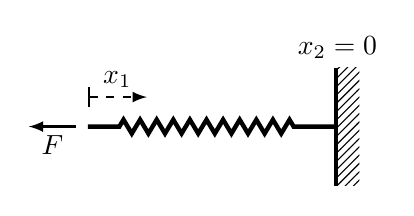
\begin{tikzpicture}[scale=1.5,xshift=0.5cm,every node/.style={outer sep=0pt,thick}]


\tikzstyle{spring}=[ultra thick,decorate,decoration={zigzag,pre length=0.4cm,post length=0.5cm,segment length=6}]

\tikzstyle{damper}=[ultra thick,decoration={markings,  
  mark connection node=dmp,
  mark=at position 0.5 with 
  {
    \node (dmp) [ultra thick,inner sep=0pt,transform shape,rotate=-90,minimum width=25pt,minimum height=8pt,draw=none] {};
    \draw [ultra thick] ($(dmp.north east)+(4pt,0)$) -- (dmp.south east) -- (dmp.south west) -- ($(dmp.north west)+(4pt,0)$);
    \draw [ultra thick] ($(dmp.north)+(0,-10pt)$) -- ($(dmp.north)+(0,10pt)$);
  }
}, decorate]

\tikzstyle{ground}=[fill,pattern=north east lines,draw=none,minimum width=2.5cm,minimum height=0.3cm]

\
\node (wall2) at (1.2cm,-4cm) [ground, rotate=90, minimum width=1.5cm] {};
\draw [ultra thick] (wall2.north east) -- (wall2.north west);
\draw [spring] (-1cm,-4cm) -- (wall2.north) node[] {};
	\draw [latex-, thick] (-1.5cm,-4cm) --  ++(0.4cm,0cm) node[pos=.5,,below] {$F$};
\draw [|-latex, thick,dashed] (-1cm,-3.75cm) -- (-0.5cm,-3.75cm) node[above,midway] {$x_1$};
\node (x0) at (wall2.south) [right,xshift=-0.9cm,yshift=1cm] {$x_2=0$};



\end{tikzpicture}

\end{document}